\section{Simulation Results}

We can now test more complex setups by doing Bit Error Rate (BER) analysis.

\begin{figure}[H]
  \centering
  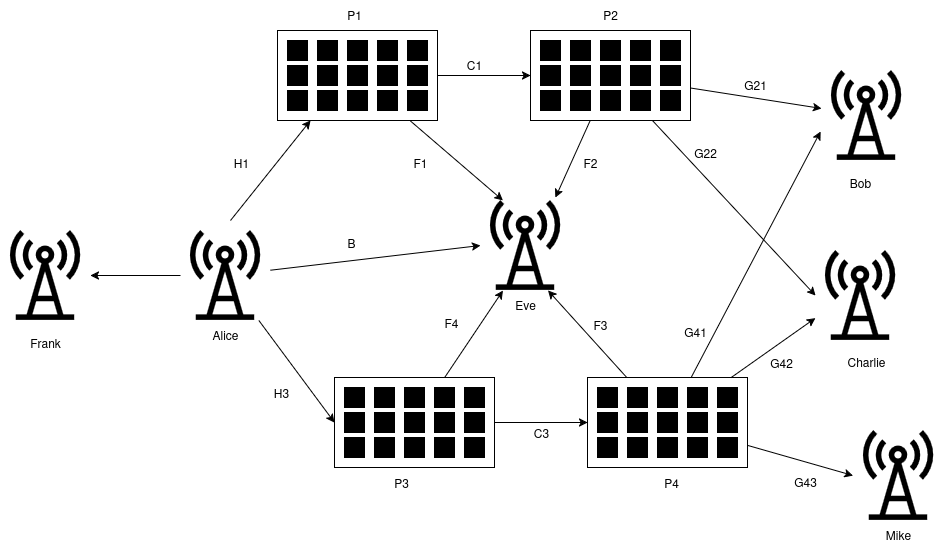
\includegraphics[width=\linewidth]{imgs/complex-situation.png}
  \caption{Complex Setup}
  \label{fig:correlation_sk2}
\end{figure}

For example, here we have a single transmitter \textit{Alice} and multiple receivers. \textit{Frank} is a direct receiver in line of sight. \textit{Bob} and \textit{Charlie} receive the signal from two double RIS reflection. \textit{Eve} receives both the direct signal and the reflecting signal from all RISs. \footnote{It should be noted that if \textit{Eve} is in the same position as \textit{Frank} and receives just the direct signal, our particular framework would not give us physical layer security, and higher layer security would be needed. If instead \textit{Eve} has not line of sight, the message would be completely unreadable from the start, since it would receive random matrixes.}

More in general, we would have $M$ consecutive RIS (in series) that reflect a signal, $J$ legitimate receivers and $Q$ different paths of RIS (in parallel) to send the signal at the same time. \footnote{The paths could have a different number of RIS (for example, a path of three and another of two). The results would still hold.}

We will show simulation results for different combinations of ($M, J$), both with a single and double path. In all scenarios, $K = 2, N = 16, \eta = 0.9$ will be the number of antennas for all actors, the number of reflecting surfaces and the reflection coefficients.

The direct link and the eavesdropper will try to understand the message by following the instructions on \cite{5165332}, while the receivers will try to understand it by following the instructions on \cite{9328149}.

\subsection{Single RIS reflection (M=1)}

\begin{figure}[H]
  \centering
  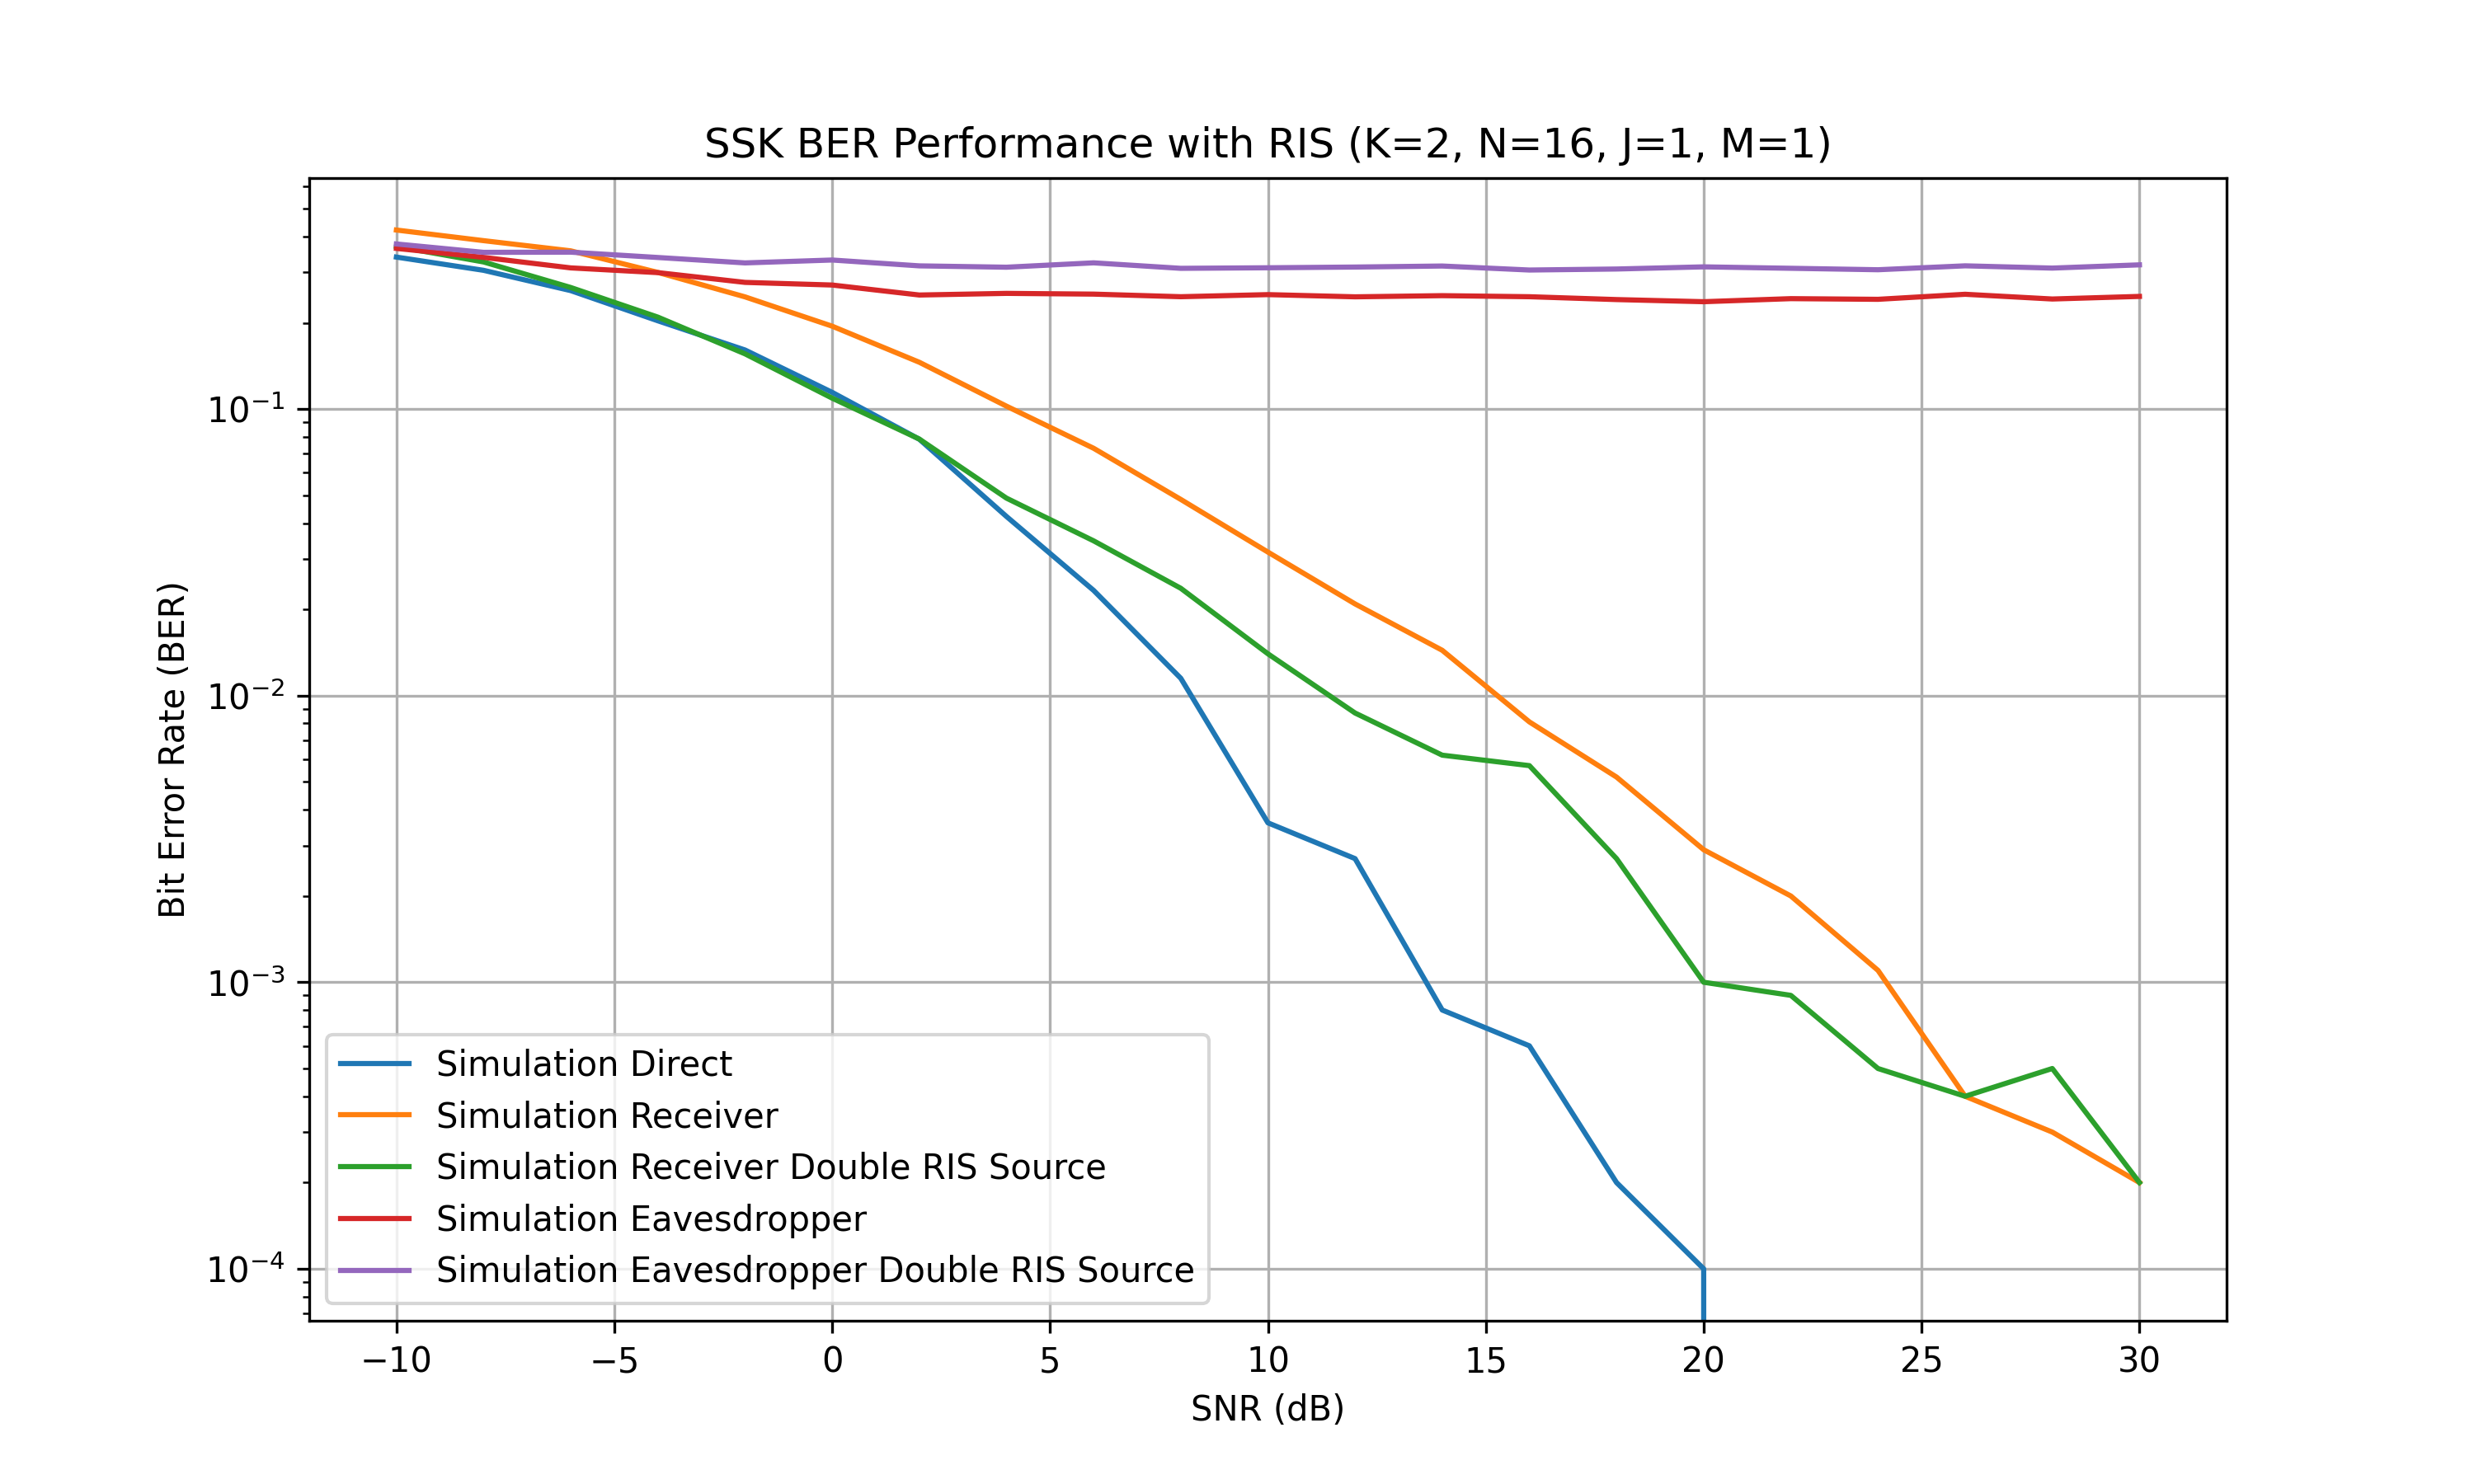
\includegraphics[width=\linewidth]{imgs/ber-simulations/SSK BER Performance with RIS (K=2, N=16, J=1, M=1).png}
  \caption{SSK BER Performance with RIS (K=2, N=16, J=1, M=1)}
  \label{fig:simulation_j1_m1}
\end{figure}

We can see in ($M=1, J=1$) the results match with \cite{9328149}, for both \textit{Simulation Receiver} and \textit{Simulation Eavesdropper}.
\textit{Simulation Direct} is the strongest possible path, mainly because of the reflection loss due to $\eta$.
Combining two different RIS in parallel (\textit{Double RIS Source}) gives better signal to the receiver, while disturbing more the signal to the eavesdropper.

\begin{figure}[H]
  \centering
  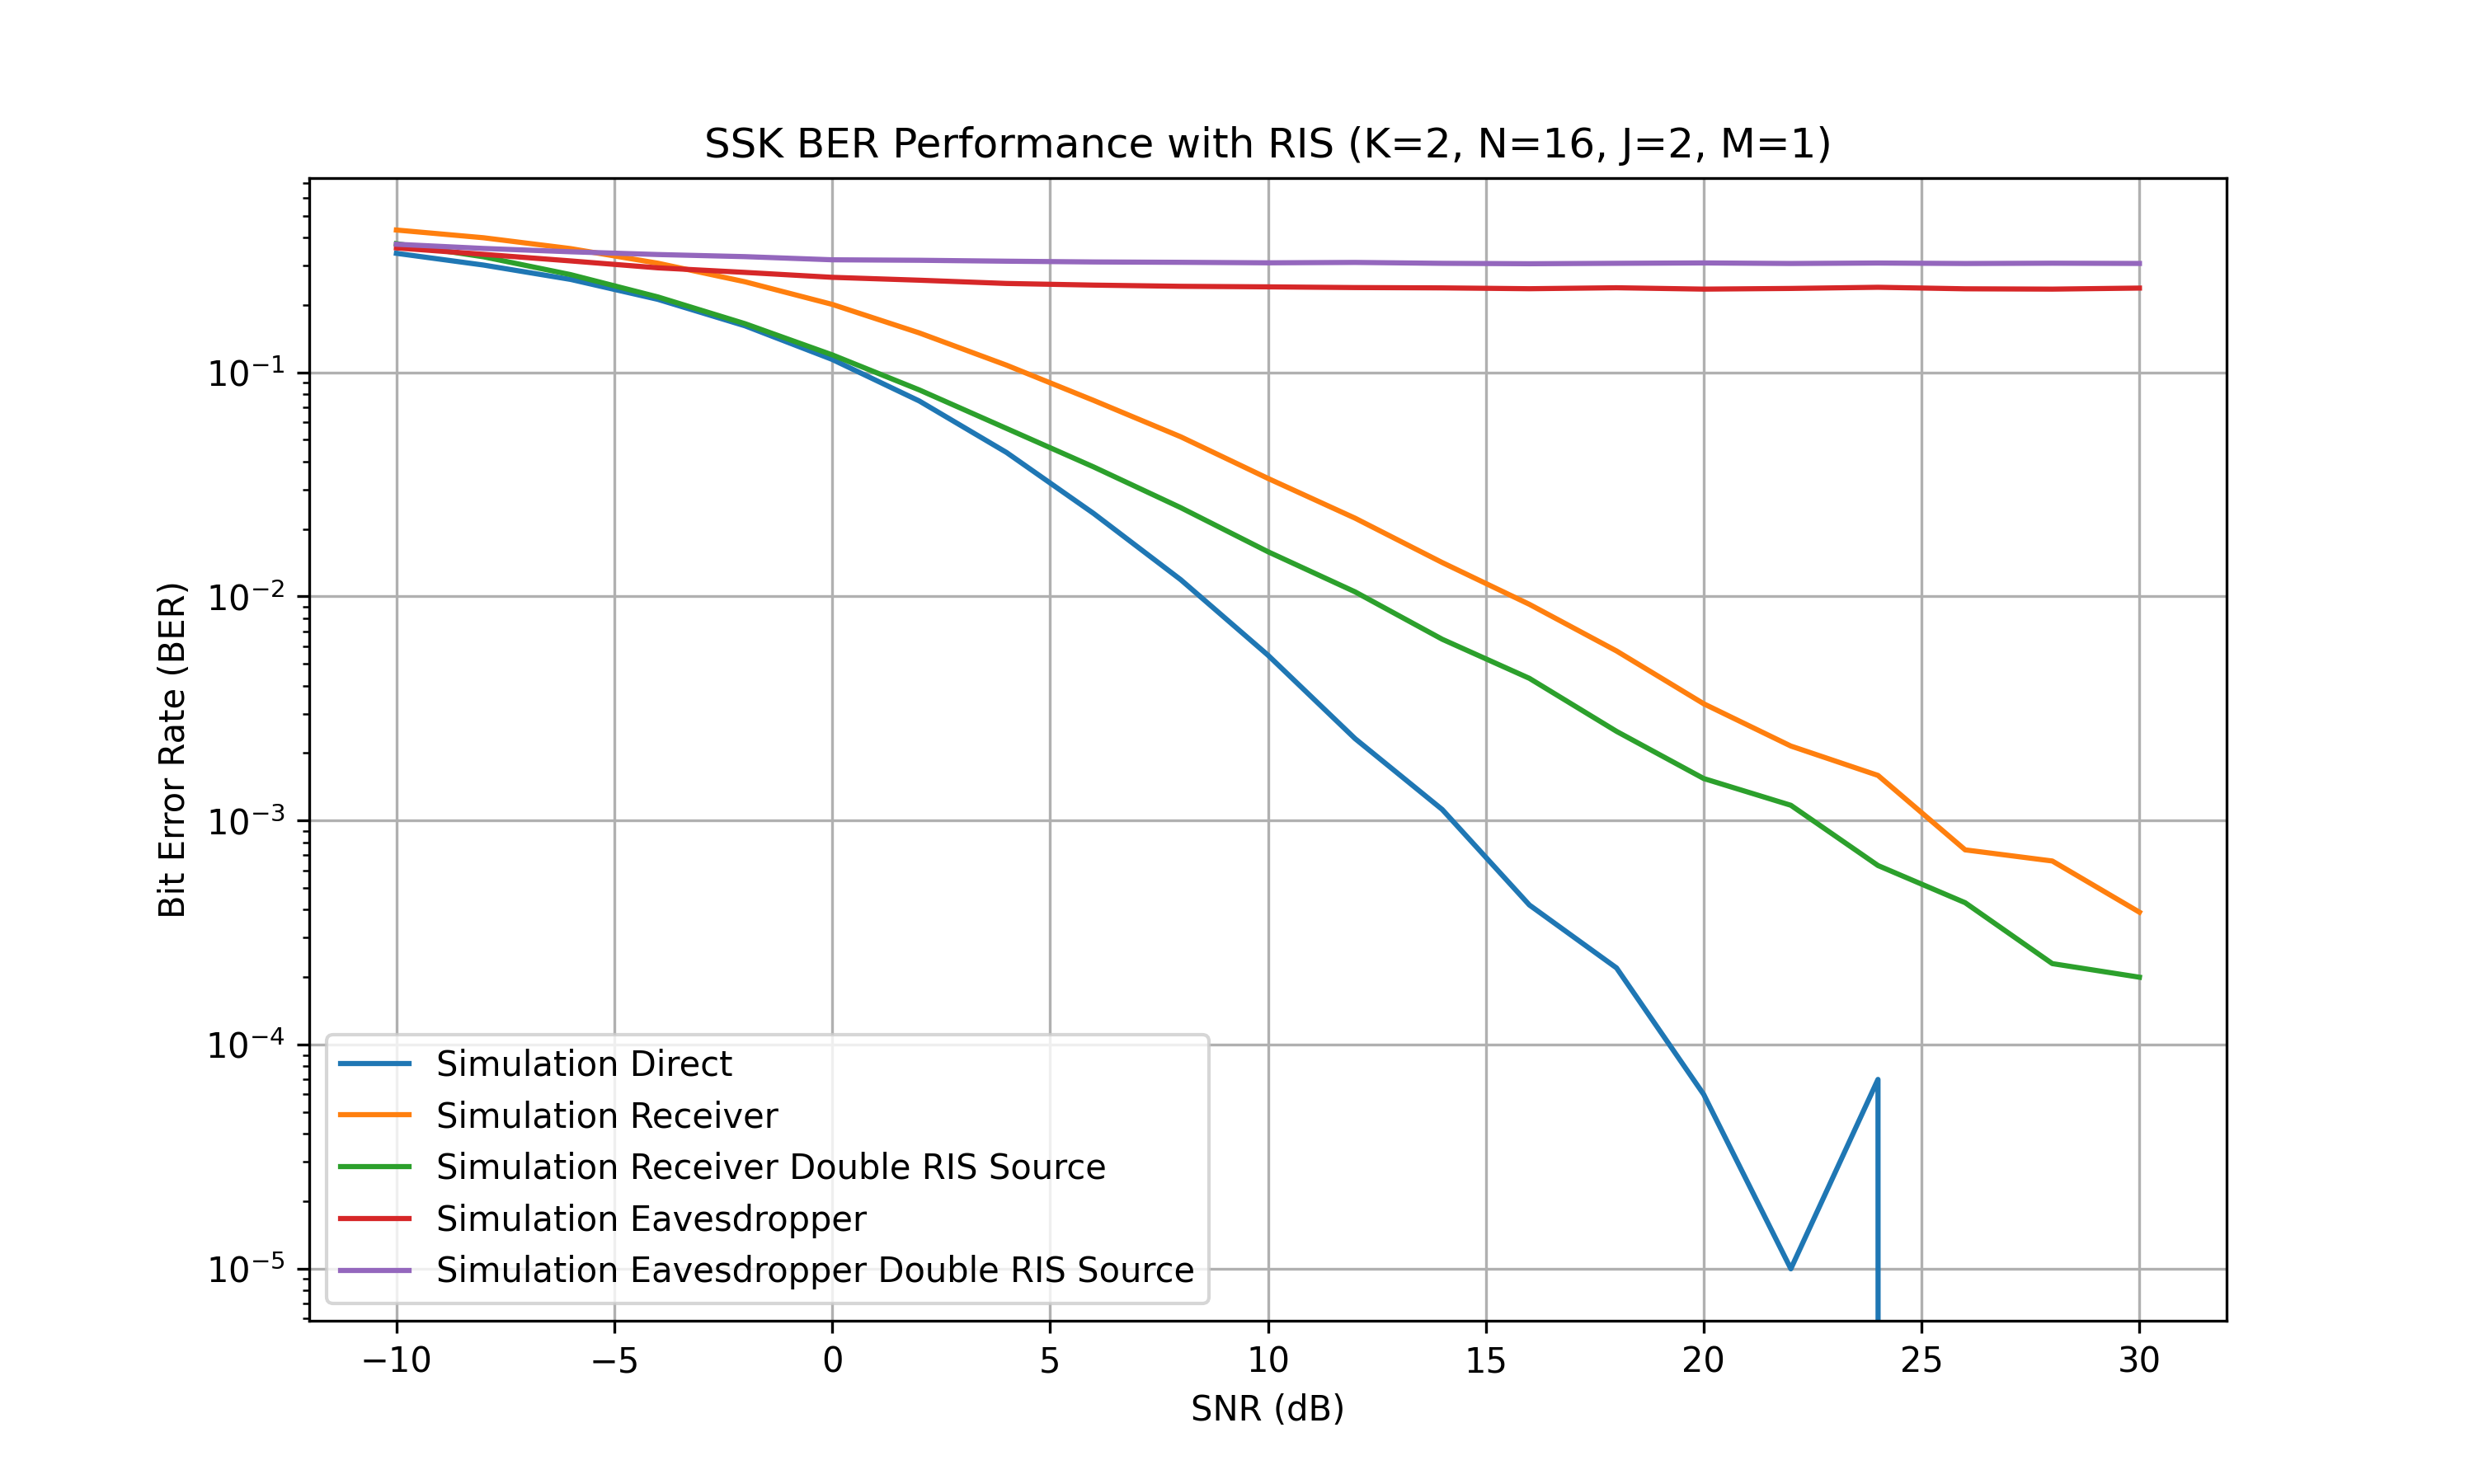
\includegraphics[width=\linewidth]{imgs/ber-simulations/SSK BER Performance with RIS (K=2, N=16, J=2, M=1).png}
  \caption{SSK BER Performance with RIS (K=2, N=16, J=2, M=1)}
  \label{fig:simulation_j2_m1}
\end{figure}

Increasing the number of receivers does not influence the result of our framework: the receivers still get a good signal depending on the SNR, while the eavesdropper is not getting an advantage in understanding the message.

\subsection{Double RIS reflection (M=2)}

\begin{figure}[H]
  \centering
  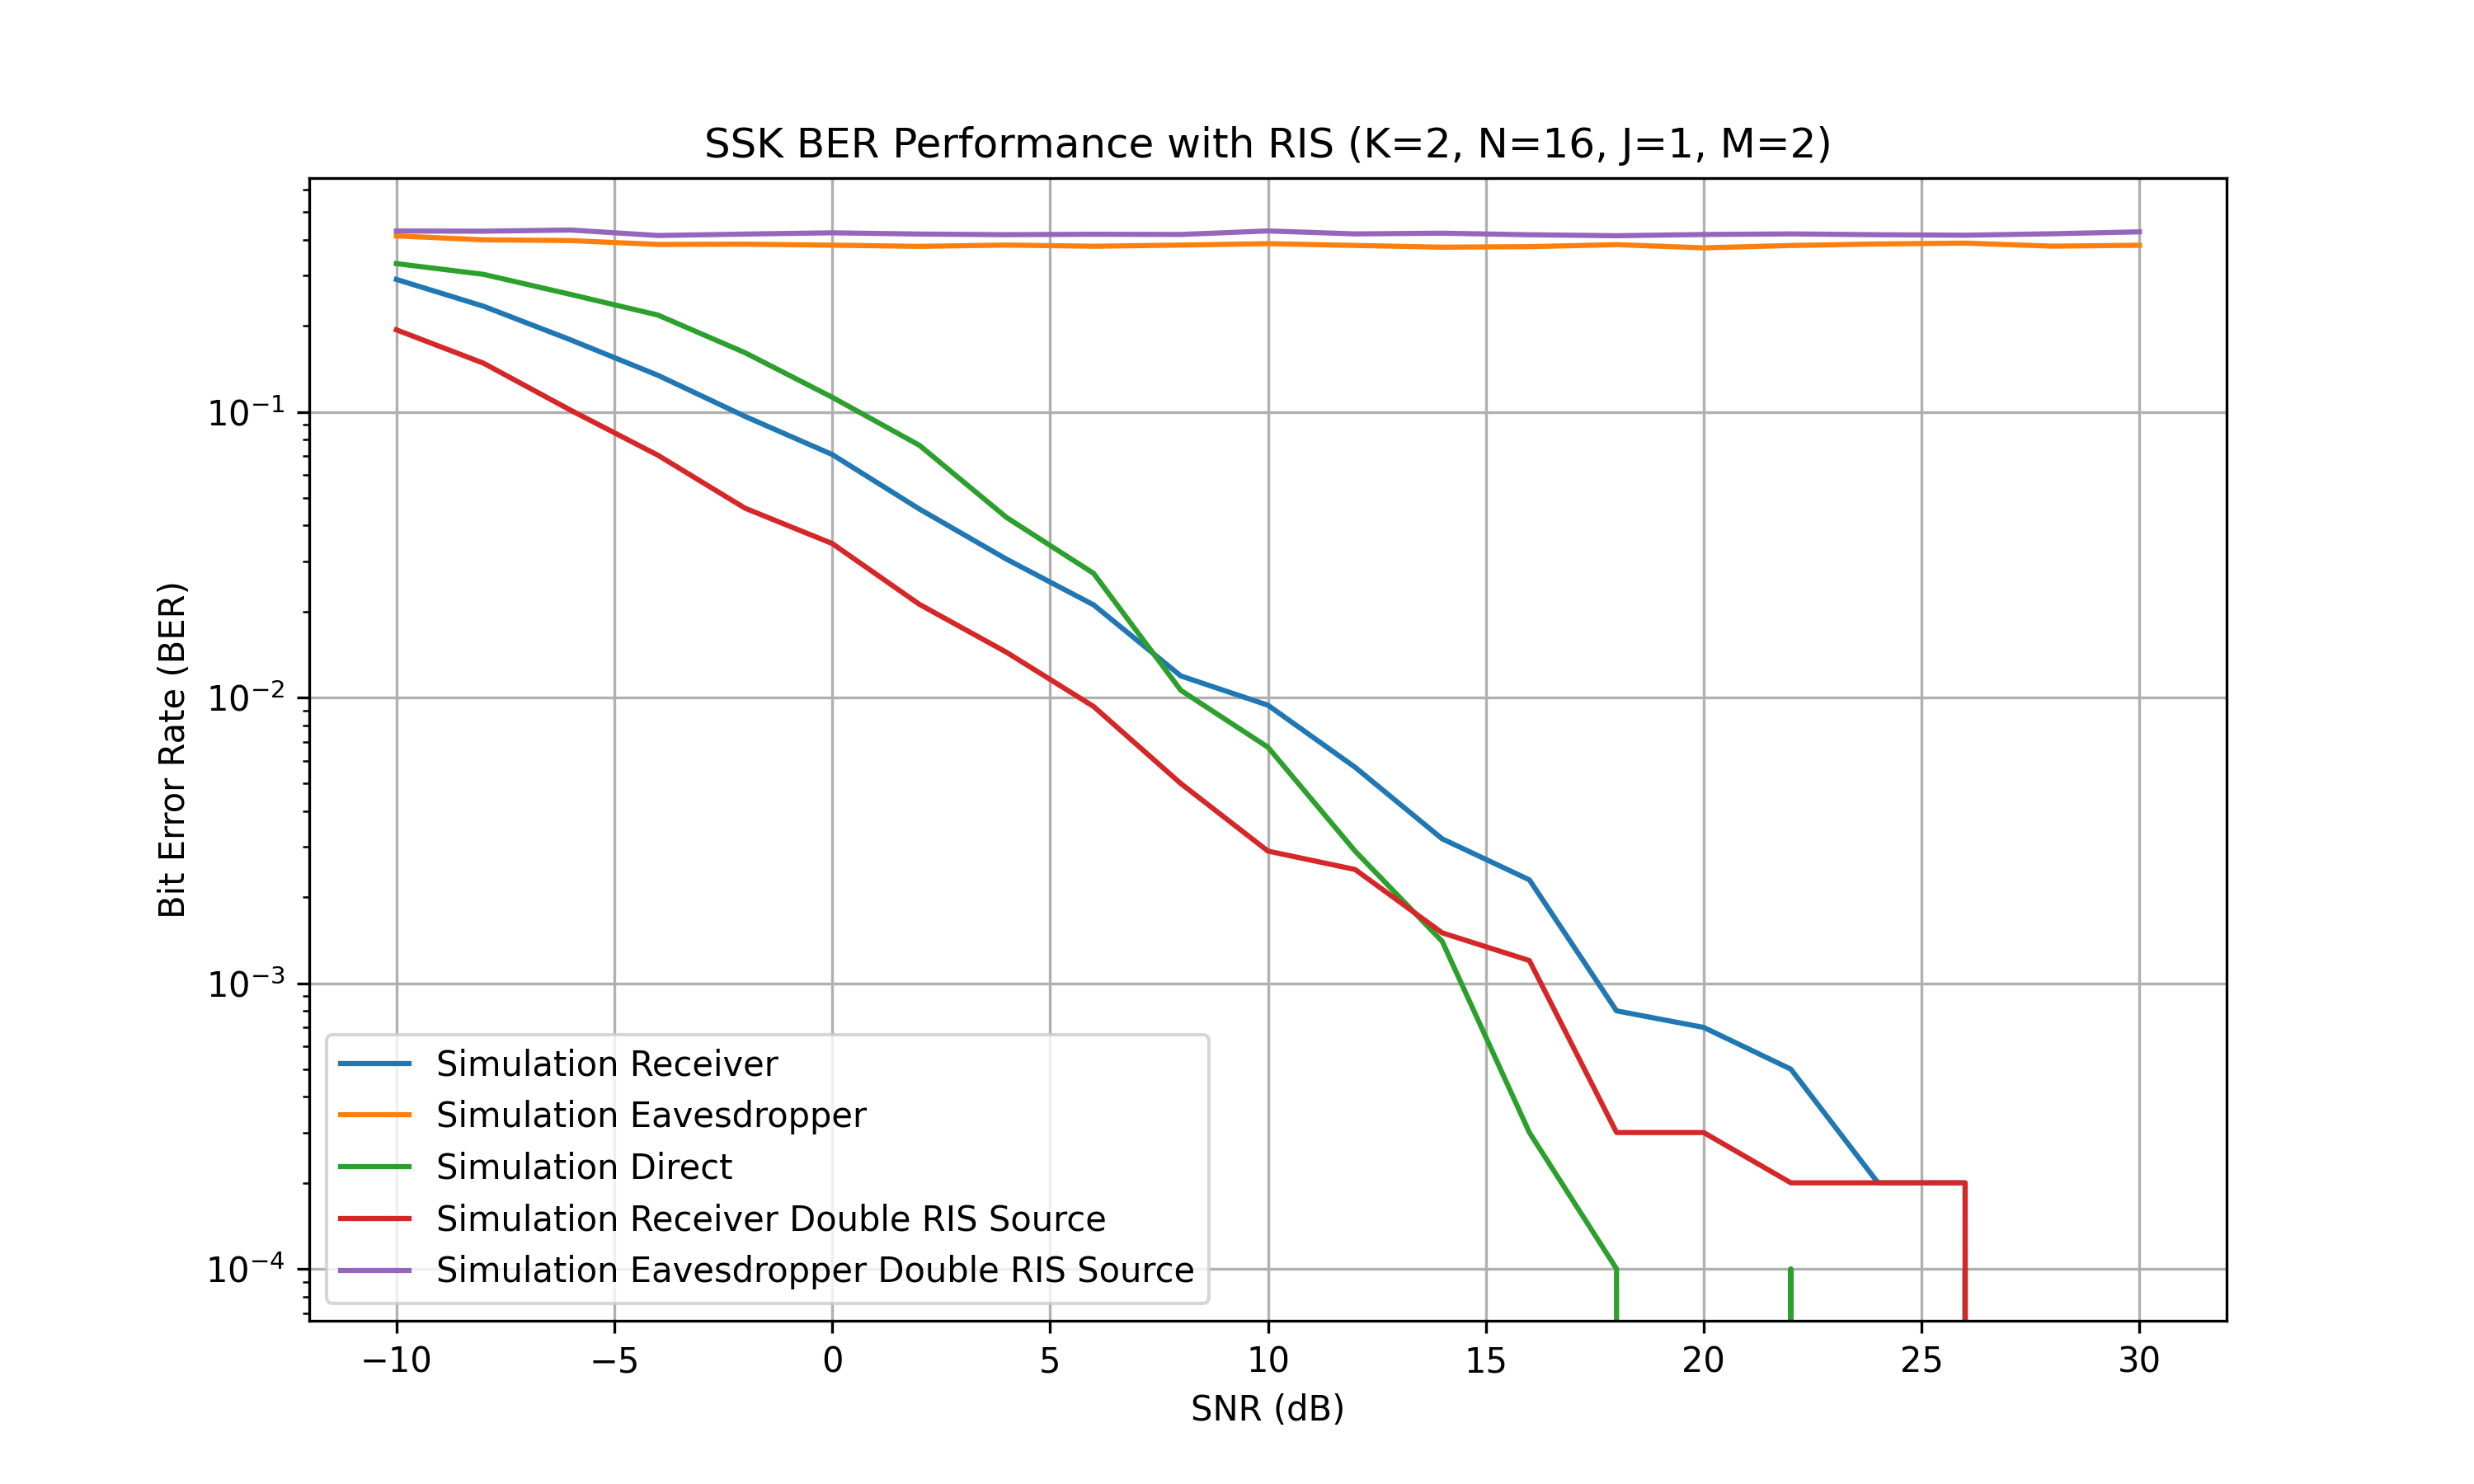
\includegraphics[width=\linewidth]{imgs/ber-simulations/SSK BER Performance with RIS (K=2, N=16, J=1, M=2).png}
  \caption{SSK BER Performance with RIS (K=2, N=16, J=1, M=2)}
  \label{fig:simulation_j1_m2}
\end{figure}

With multiple RIS in series, the eavesdropper get a worse signal because of the double interference of the 2 RIS.
\textbf{(TODO: Why the receiver is getting a better signal? Should it not be worse? Check normalization of the signal)}

\begin{figure}[H]
  \centering
  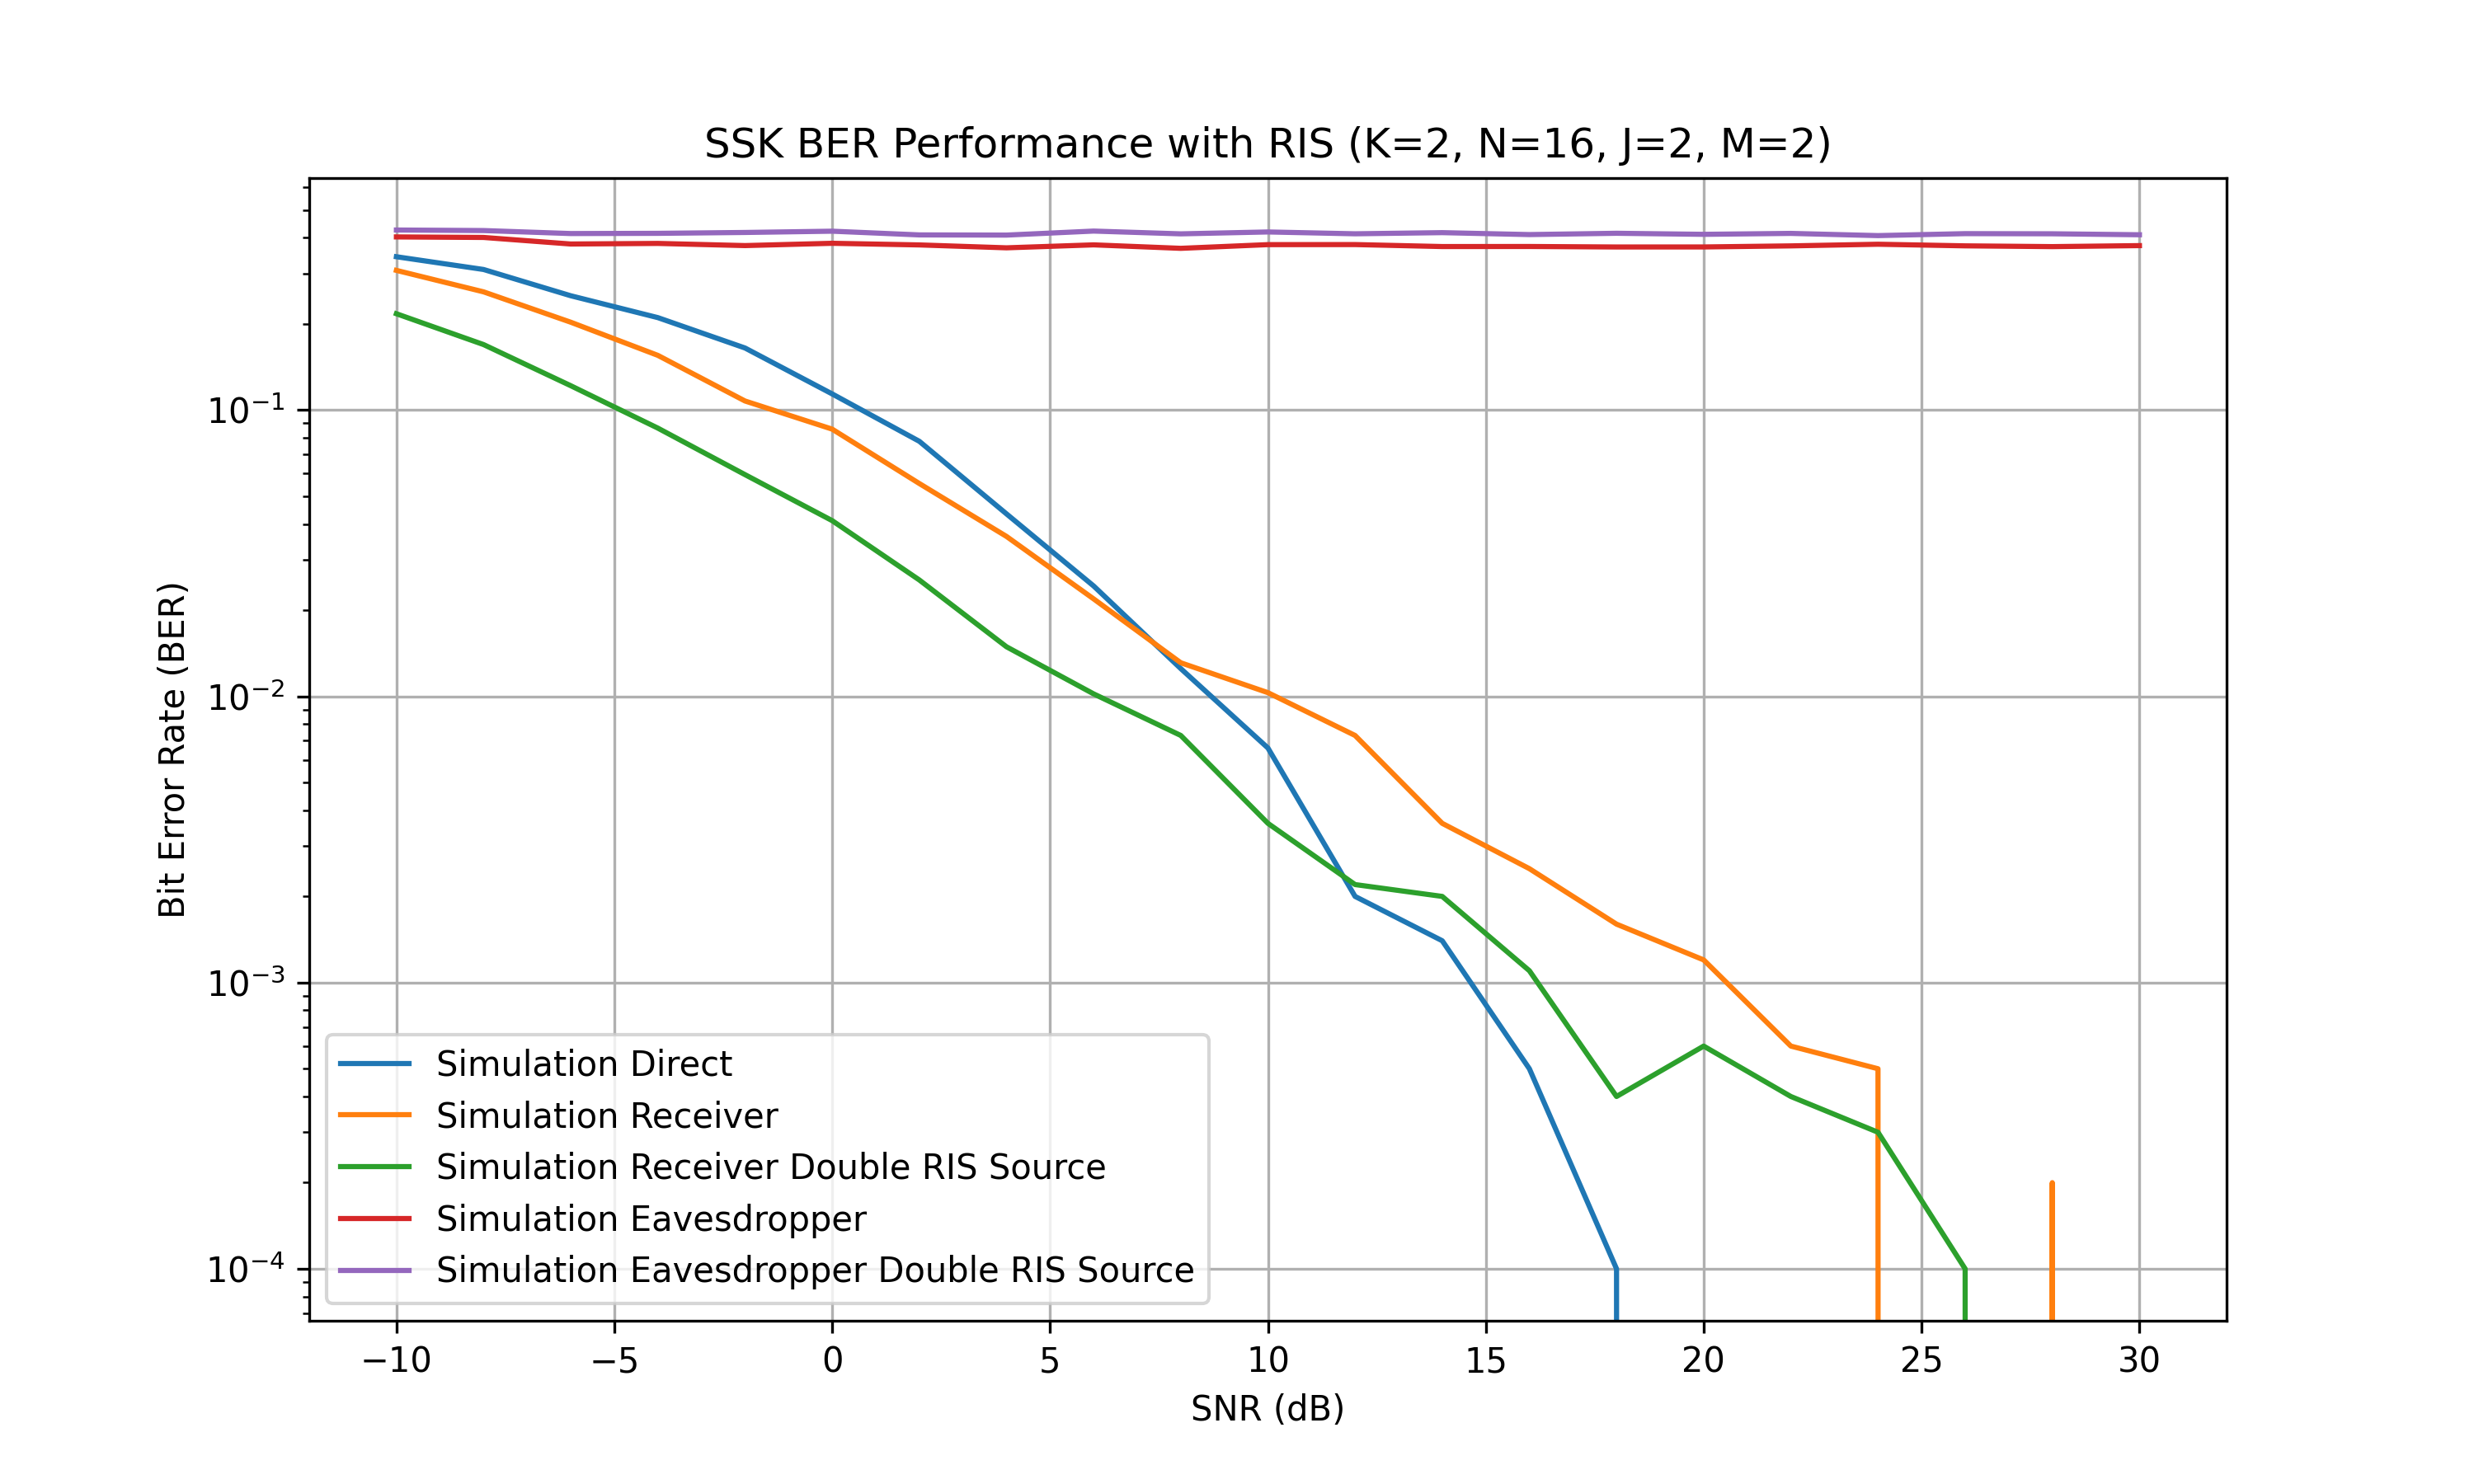
\includegraphics[width=\linewidth]{imgs/ber-simulations/SSK BER Performance with RIS (K=2, N=16, J=2, M=2).png}
  \caption{SSK BER Performance with RIS (K=2, N=16, J=2, M=2)}
  \label{fig:simulation_j2_m2}
\end{figure}

Combining all together, our properties still hold strong.